%% TODO: Make sure to use \textbf or \textit for highlighting keywords, and \cite{} to cite the corresponding quotations
\section{Overview}

\hspace{0.5cm}The methodology chapter provides a comprehensive overview of the approach taken in this research. It outlines the key components of the system, including the Business Logic Analyzer module (BLA), the AI-integrated test generation module, and the AI test validation module. Each component is designed to work seamlessly together, leveraging Python, Flask, and Langchain to create an efficient and effective solution for automating test case generation. The chapter also discusses the methods implemented for each module and the plan to validate the generated tests from AI, ensuring that the proposed solution meets its objectives and addresses the identified challenges in software testing.
\section{User requirement analysis}

\hspace{0.5cm}Understanding user requirements is a critical step in ensuring that the proposed system aligns with the needs and expectations of its target audience. This phase involves identifying and analyzing the specific functionalities, constraints, and preferences that users demand from the system. A thorough understanding of user requirements not only guides the development process but also ensures the system delivers value by addressing real-world challenges effectively. This section outlines the key user requirements identified for the proposed test generation service.

% table of 4 columns: Req.ID, Requirement Name, Detailed Description, Type
\begin{table}[H]
	% margin right a little
	% \hspace{-1cm}
	\centering
	\begin{tabular}{|c|p{110pt}|p{8cm}|p{62pt}|}
		\hline
		\textbf{Req.ID} & \textbf{Requirement Name} & \textbf{Detailed Description} & \textbf{Type} \\ \hline
		001 & Read project's source code & Users can send all project's source code at once via web-based Git repositories (e.g github, gitlab) & Functional requirement \\ \hline
		002 & Download/copy unit test/integration test & Users can download tests files or copy the file's content. & Functional requirement \\ \hline
		003 & Interactive business logic analyzation (Human-inner-loop) & Users can help AI correct the result of BLA process & Functional requirement \\ \hline
		004 & Performance & The system should generate test cases within a reasonable time frame, ideally under 5 minutes for a medium-sized project (e.g., 10,000 lines of code). & Non-functional requirement \\ \hline
		005 & Test file correctly reflect the given business model & The system should be able to generate test cases accurately reflect the business logic embedded in the source code. & Non-functional requirement \\ \hline
		006 & Validate generated test & A validation mechanism must be included to the system to ensure the syntax and logic is runnable & Non-functional requirement \\ \hline
	\end{tabular}
	\caption{User requirements}
	\label{tab:user-requirements}
\end{table}

\subsection{Ability to send project's source code}
\hspace{0.5cm}The Test Genie system requires users to submit their project's source code via web-based Git repositories (e.g., GitHub, GitLab) rather than traditional methods like ZIP files. This design is intentional and aligns with modern development workflows since most modern projects have an online git repository. The biggest advantage is that this method will optimize unneeded directory that will be added to gitignore by users. Some modern framework use library that is sometimes heavy and not necessary during Business Logic Analyze process. Not adding these files will optimize the workloads of system much better.

\hspace{0.5cm}\textbf{User flow.}	Users will input the Git repository link via the User Interface (UI) and select the desired branch for analysis. If the system encounters access issues or cannot connect to the repository (e.g., internal Git systems), it will respond with an error message, prompting the user to resolve the issue.

\hspace{0.5cm}\textbf{System flow.}    After receiving the Git link and branch information, the system will clone the repository. Using predefined tokens or configuration files (e.g., pubspec.yaml for Flutter), the system will identify the framework and dependencies used in the project. Based on this information, the system will apply the most suitable strategy to analyze the source code and generate test cases.

\subsection{Give user output}

\hspace{0.5cm}The output of the system is a full test file content that can be integrate into their existing workflows. The output is delivered through a live chat downloadable UI, ensuring a seamless and interactive experience for users.

\hspace{0.5cm}\textbf{Output format.} Currently, this system only supports the Flutter framework, which has a built-in testing system. The system generates test files with the naming convention \textit{“filename\_test.dart”}, where the filename corresponds to the specific module or functionality being tested. This naming convention ensures that the test files are easily identifiable and organized within the project structure. The content of the test files is tailored to match the testing requirements requested by the user, including unit tests, integration tests, or widget tests, depending on the analysis of the source code. By adhering to Flutter's testing standards, the generated files are immediately compatible with the framework, allowing developers to run the tests without additional configuration. This approach ensures that the output is not only functional but also aligns with best practices for Flutter development.

\hspace{0.5cm}\textbf{Live chat interface.}     Users receive the generated test files through a live chat interface embedded in the system's UI. This interface provides a real-time, interactive experience, enabling users to communicate with the system as it generates and refines test cases. For example, if the user identifies an issue with the generated tests (e.g., incorrect logic, missing edge cases, or mismatched parameters), they can provide feedback directly through the chat. The system will then process this feedback and adjust the test cases accordingly. This two-way communication ensures that the final output meets the user's expectations and aligns with the project's requirements. Additionally, the live chat interface can provide explanations or suggestions for improving the tests, making it a valuable tool for both novice and experienced developers. This interactive approach enhances user satisfaction and ensures that the generated tests are accurate and relevant.

\hspace{0.5cm}\textbf{Downloadable Files.}     Instead of requiring users to manually create and organize test files, the system allows users to download the generated files directly and save them in the /tests/ folder of their Flutter project. This feature eliminates the need for manual file creation and ensures that the tests are placed in the correct directory, adhering to Flutter's project structure. The files are packaged in a format that is ready to be integrated into the user's project, requiring minimal manual intervention. This seamless integration reduces the risk of errors and saves developers' valuable time. Furthermore, the system ensures that the downloaded files are compatible with version control systems like Git, allowing users to immediately commit the tests to their repository. This feature is particularly useful for teams working in collaborative environments, as it streamlines the process of adding tests to the codebase.

\hspace{0.5cm}\textbf{Easy to adjust.}	Although the system is embedded with a validator to ensure that the generated tests are syntactically correct and runnable, it recognizes that real-world scenarios may require adjustments. For instance, the system might generate tests based on default parameters or assumptions that do not fully align with the user's specific use cases. In such situations, users can easily adjust the test parameters to better fit their requirements. The system provides clear and well-structured test files, making it straightforward for developers to modify variables, inputs, or assertions as needed. This flexibility ensures that the generated tests remain useful even in complex or unique scenarios. By combining automated test generation with the ability to manually refine the results, the system strikes a balance between efficiency and adaptability, catering to a wide range of development needs.

\subsection{Interactive Business Logic Analyzating process}

\hspace{0.5cm}The Business Logic Analyzing (BLA) process plays a crucial role in ensuring that the system accurately interprets and applies business logic. If the output of this process is incorrect, it can lead to downstream malfunctions and errors, which can be costly and time-consuming to resolve. To address this, the system incorporates an interactive BLA process that allows users to collaborate with the AI to improve analysis results.

\hspace{0.5cm}\textbf{User interface.}	The interface for this process is designed to be intuitive and user-friendly, enabling users to interact with a visual representation of the project's modules, classes, and functions in the form of a graph. This graphical layout provides a clear overview of how different components of the application are interconnected and functioned. Users can inspect the analysis results by interacting with this graph, allowing them to identify potential issues or discrepancies in the current output.

\hspace{0.5cm}One key feature of this interface is its ability to be manipulated by users. Through inspection, users can help guide the AI by highlighting specific areas of interest, providing context, or pointing out errors in the analysis. This interactive capability allows for a more precise and accurate understanding of how the business logic is being applied within the system.

\hspace{0.5cm}\textbf{Sytem flow.}	Once the project's source code has been submitted to the system, it undergoes an initial analysis phase that maps out the relationships between classes, modules, and functions. The system uses this information to generate a detailed breakdown of the project's structure and flow. After the analysis is complete, users receive access to a project insight webview that provides a comprehensive visual representation of how these components interact with each other.

\hspace{0.5cm}This webview not only displays the flow of the project but also highlights any potential issues or areas where the business logic may require adjustment. The system ensures that this visualization is clear and concise, making it easy for users to understand and address any discrepancies in the analysis.

\subsection{Optimize performance}

\hspace{0.5cm}The input of this system is the user’s source code of the project they needed to generate. A study show that the average number lines of code (LOC) of a project with 90 functions will have 90,000 lines of codes [10]. From AI perspective, that is an enormous amount of input tokens. To handle these input lighter, these inputs will be split into blocks of component to analyze.

\hspace{0.5cm}\textbf{Splitting strategy.}		In this system, relational database will be used to store project’s source code. Each component will contain the input, output, related component information and the predicted business logic of that component. This structured approach allows for efficient handling and analysis of large inputs while maintaining clarity and organization.

\hspace{0.5cm}\textbf{Quering component.}		The graphical webview that was introduced above will be contruct by query the connection of these component. 

\hspace{0.5cm}\textbf{Performance overall.}	By organizing the input into blocks of component and using efficient querying mechanisms, the system optimizes its ability to handle large-scale projects without compromising performance. The use of a relational database ensures that data retrieval is both organized and efficient, reducing the likelihood of bottlenecks during analysis.

\hspace{0.5cm}This approach not only enhances the system's capacity to process extensive codebases but also improves overall efficiency by minimizing redundant data storage and retrieval processes.

\subsection{Good test file generation - Quality control}

\hspace{0.5cm}To ensure high-quality test file generation while maintaining the abstraction of the LLM model, this thesis adopts the Retrieval-Augmented Generation (RAG) technique. This approach involves embedding relevant project framework documents (currently focused on Flutter) and providing them as input to the model through structured prompts. By augmenting the model with specific, context-rich information, the system can generate test cases that better align with the framework’s requirements and coding standards.

\hspace{0.5cm}\textbf{Provided documents.}	The documents supplied to the LLM are carefully selected to include essential information related to testing syntax, techniques, and best practices for the Flutter framework. These resources guide the model in generating syntactically correct and framework-compliant test cases.

\hspace{0.5cm}\textbf{User-side documents.}	Users have the option to provide supplementary documents and sample test files from their projects. This customization allows the system to learn and adhere to the specific naming conventions, organizational structures, and testing styles already established within the project.

\subsection{Test validation}

\hspace{0.5cm}In this thesis, the validation scope focuses on ensuring that the generated test files are runnable within the intended development environment. Rather than validating the correctness of test outcomes or the business logic they cover, the emphasis is placed on generating test files that can be successfully executed without syntax or framework-related errors.
To achieve this, a Software Development Kit (SDK) is embedded for each supported framework, with the initial implementation targeting the Flutter framework. This SDK integration ensures compatibility with the framework's testing infrastructure, allowing the generated tests to be seamlessly executed as part of the development workflow. By embedding the SDK, the system can identify and address potential issues during the test generation process, such as missing dependencies or incorrect file structures, thereby increasing the reliability of the output.
\hspace{0.5cm}While the current scope does not extend to evaluating the correctness of test assertions or coverage, this foundational validation approach ensures that developers receive test files that are syntactically correct, executable, and immediately ready for further refinement or deployment within their projects. Future enhancements may involve integrating more advanced validation techniques, such as logic verification 

\section{System Design}

\subsection{Core Design Philosophy}

\hspace{0.5cm}The fundamental challenge in AI-based test generation is source code bias, where the AI model's exposure to implementation details leads to tests that merely replicate code behavior rather than validating business requirements. Test Genie addresses this challenge through a novel architectural approach based on modular analysis and isolation of concerns.

\hspace{0.5cm}Source code bias occurs when an AI model, given complete access to implementation details, generates tests that are essentially tautological—they validate that the code does what the code does, rather than what it should do according to business logic. This issue undermines the purpose of testing as an independent verification mechanism. Traditional approaches either restrict AI access to implementation details (limiting effectiveness) or accept this bias as inevitable.

\hspace{0.5cm}Test Genie's approach is fundamentally different. By decomposing source code into discrete, semantically meaningful blocks and analyzing them in isolation, the system creates a separation between implementation and testing concerns. Each block represents a distinct functional unit with clear inputs, outputs, and business logic implications. This decomposition allows the system to:

\begin{itemize}
    \item Generate accurate predictions about each block's purpose without being overwhelmed by the complexity of the entire codebase
    \item Focus on functional intent rather than implementation details
    \item Isolate business logic from technical implementation
    \item Enable effective human-in-the-loop correction at a manageable granularity
\end{itemize}

\hspace{0.5cm}This modular approach offers significant advantages over traditional methods. While conventional test generation might produce tests that trivially pass because they mirror the implementation logic, Test Genie's block-based analysis encourages tests that validate the expected behavior of each component according to its business purpose. Figure~\ref{fig:system-design} visualizes this architectural philosophy, showing how decomposition into blocks enables more effective analysis and test generation.

\subsection{System Architecture}

\hspace{0.5cm}The Test Genie system implements a three-tier architecture consisting of the \textbf{User Interface (UI)}, the \textbf{Request Handler} middleware, and the \textbf{Application Service (Backend)} layer. This architecture facilitates clear separation of concerns, enabling each component to fulfill its specific role in addressing the source code bias problem. Figure~\ref{fig:system-design} illustrates the overall module design of the system.

\begin{figure}[H]
	\centering
	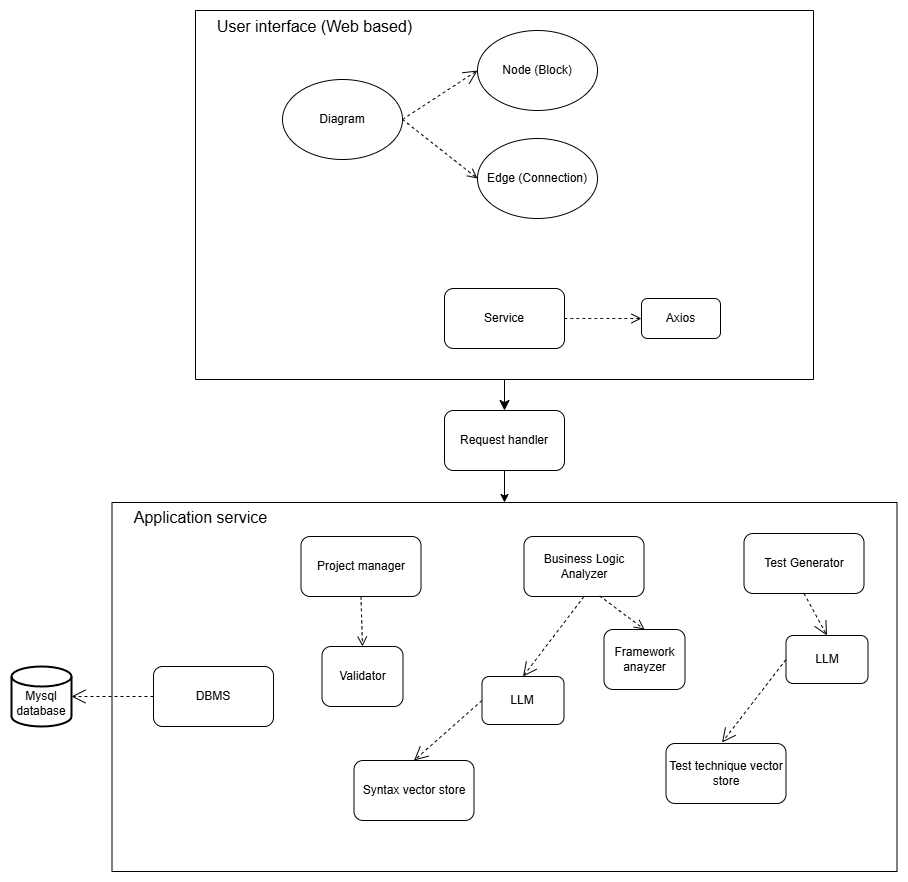
\includegraphics[width=1.0\textwidth]{images/System design.drawio.png}
	\caption{Test Genie's overall module design}
	\label{fig:system-design}
\end{figure}

\subsubsection{User Interface (UI) Layer}

\hspace{0.5cm}The User Interface layer serves as the primary interaction point between users and the Test Genie system. Built as a web-based application, it combines visualization capabilities with interactive elements designed specifically to facilitate human-in-the-loop participation in the analysis and test generation process. Key components include:

\begin{itemize}
    \item \textbf{Interactive Graph Visualization}: Renders the source code structure as a navigable graph of blocks and connections, allowing users to visually comprehend complex project architectures. The visualization employs force-directed graph algorithms to optimally arrange components based on their interconnections.
    
    \item \textbf{Block Inspector}: Provides detailed views of individual code blocks, including:
    \begin{itemize}
        \item \textbf{Source Code View}: Syntax-highlighted representation of the block's actual implementation
        \item \textbf{Prediction Editor}: Interactive interface for viewing and refining the AI-generated predictions about the block's business purpose
        \item \textbf{Test Preview}: Live preview of generated test cases with syntax highlighting
    \end{itemize}
    
    \item \textbf{Human-in-the-Loop Controls}: Interface elements that enable users to:
    \begin{itemize}
        \item Navigate between related blocks and understand their connections
        \item Modify AI-generated predictions when they misinterpret business logic
        \item Trigger test regeneration after prediction updates
        \item Download or copy generated test files
    \end{itemize}
\end{itemize}

\hspace{0.5cm}The UI is designed with a focus on transparency and interpretability, allowing users to understand and influence the AI's reasoning process. This transparency directly addresses the source code bias problem by enabling users to identify and correct cases where the AI has focused too heavily on implementation details rather than business intent. By providing visual representation of blocks and their relationships, the UI helps users mentally separate implementation from specification, reinforcing the system's core philosophy.

\subsubsection{Request Handler Layer}

\hspace{0.5cm}The Request Handler layer serves as the communication bridge between the UI and backend services, implementing a RESTful API architecture that processes user interactions and coordinates system responses. This layer implements several key functions:

\begin{itemize}
    \item \textbf{Request Routing and Validation}: Ensures that user requests are well-formed and directed to the appropriate backend services
    
    \item \textbf{Caching and Performance Optimization}: Maintains a cache of frequently accessed data to minimize redundant computation and database queries
    
    \item \textbf{Session Management}: Tracks user sessions and maintains contextual information about ongoing analysis tasks
    
    \item \textbf{Response Formatting}: Transforms backend results into structured data formats suitable for UI presentation
\end{itemize}

\hspace{0.5cm}Table~\ref{tab:api-endpoints} outlines the primary API endpoints implemented by the Request Handler layer:

\begin{table}[H]
	\centering
	\begin{tabular}{|l|p{3cm}|p{8cm}|}
		\hline
		\textbf{Endpoint} & \textbf{Method} & \textbf{Purpose} \\ \hline
		/createProject & POST & Initialize project analysis by providing Git repository URL \\ \hline
		/getDiagram & POST & Retrieve block and connection data for visualization \\ \hline
		/getBlockContent & POST & Fetch source code and metadata for a specific block \\ \hline
		/getBlockDetail & POST & Retrieve comprehensive information about a block, including predictions and tests \\ \hline
		/getBlockPrediction & POST & Retrieve the current business logic prediction for a block \\ \hline
		/updateBlockPrediction & POST & Update the business logic prediction for a block based on user input \\ \hline
		/generateTest & POST & Generate test cases for a specified block using current predictions \\ \hline
	\end{tabular}
	\caption{Request Handler API Endpoints}
	\label{tab:api-endpoints}
\end{table}

\hspace{0.5cm}The Request Handler's implementation of these endpoints ensures that user interactions with the UI efficiently translate to appropriate actions in the backend services. This layer's design is critical to maintaining the system's responsiveness during the iterative process of analysis, prediction refinement, and test generation.

\subsubsection{Application Service (Backend) Layer}

\hspace{0.5cm}The Backend layer contains the system's core functionality, implementing the computational processes that analyze source code, generate predictions, and create test cases. This layer comprises several specialized modules working in concert:

\paragraph{Project Manager}
\hspace{0.5cm}The Project Manager module serves as the gateway to source code analysis, with responsibilities including:

\begin{itemize}
    \item \textbf{Repository Handling}: Cloning Git repositories, managing local copies, and extracting relevant files
    
    \item \textbf{Framework Detection}: Identifying the programming framework (currently focusing on Flutter) by analyzing project structure and configuration files
    
    \item \textbf{Source File Extraction}: Identifying and extracting source files relevant for analysis while filtering out non-essential files
    
    \item \textbf{Test Environment Setup}: Creating and maintaining isolated environments for test execution and validation
    
    \item \textbf{Test Execution}: Running generated tests against the embedded framework SDK to validate correctness
\end{itemize}

\hspace{0.5cm}The Project Manager implements framework-specific adapters (currently Flutter) that encapsulate knowledge about project structures, file organizations, and testing conventions. This approach allows for future extensibility to additional frameworks while maintaining a consistent interface for other system components.

\paragraph{Business Logic Analyzer (BLA)}
\hspace{0.5cm}The Business Logic Analyzer represents the system's analytical core, implementing the block-based decomposition approach central to Test Genie's design philosophy. The BLA performs several critical functions:

\begin{itemize}
    \item \textbf{Source Code Parsing}: Converting raw source files into abstract syntax trees (ASTs) that can be analyzed programmatically
    
    \item \textbf{Block Identification}: Applying heuristic algorithms to identify semantically meaningful code blocks such as methods, functions, and classes
    
    \item \textbf{Connection Analysis}: Determining relationships between blocks based on method calls, inheritance, and other dependencies
    
    \item \textbf{Block Prediction Generation}: Applying AI analysis to each individual block to predict its business purpose
\end{itemize}

\hspace{0.5cm}The BLA's block identification process employs a specialized algorithm designed to identify code units that represent discrete functional components with well-defined inputs and outputs. This decomposition is central to addressing source code bias, as it allows the system to analyze each component's intended purpose without being overwhelmed by implementation details of the entire codebase.

\hspace{0.5cm}Algorithm~\ref{alg:block-identification} outlines the block identification process:

\begin{algorithm}[H]
	\small
	\caption{BlockIdentification(SourceFiles)}
	\label{alg:block-identification}
	\begin{algorithmic}[1]
		\Require $SourceFiles$ is a list of source code files from the project
		\State $Blocks \gets \emptyset$ \Comment{Initialize empty block collection}
		\State $Connections \gets \emptyset$ \Comment{Initialize empty connections collection}
		\For{each $file \in SourceFiles$}
		    \State $ast \gets ParseSourceToAST(file)$
		    \State $fileBlocks \gets ExtractBlocksFromAST(ast)$
		    \For{each $block \in fileBlocks$}
		        \State $block.id \gets GenerateUniqueIdentifier()$
		        \State $block.name \gets ExtractBlockName(block)$
		        \State $block.type \gets DetermineBlockType(block)$
		        \State $block.content \gets ExtractSourceCode(block)$
		        \State $block.originalFile \gets file.path$
		        \State $Blocks \gets Blocks \cup \{block\}$
		    \EndFor
		    \State $fileConnections \gets IdentifyConnectionsInFile(fileBlocks)$
		    \State $Connections \gets Connections \cup fileConnections$
		\EndFor
		\State $crossFileConnections \gets IdentifyCrossFileConnections(Blocks)$
		\State $Connections \gets Connections \cup crossFileConnections$
		\For{each $block \in Blocks$}
		    \State $block.prediction \gets GeneratePrediction(block, Blocks, Connections)$
		\EndFor
		\State \Return $(Blocks, Connections)$
	\end{algorithmic}
\end{algorithm}

\hspace{0.5cm}The prediction generation process employs an AI-based approach that combines contextual understanding with code analysis, leveraging language models enhanced with domain-specific knowledge of programming patterns and testing techniques.

\paragraph{Test Generator}
\hspace{0.5cm}The Test Generator module transforms business logic predictions into executable test cases tailored to the specific framework (currently Flutter/Dart). Key features include:

\begin{itemize}
    \item \textbf{Context-Aware Test Creation}: Generating tests that validate business requirements rather than implementation details
    
    \item \textbf{Test Framework Integration}: Producing tests compatible with the target framework's testing infrastructure
    
    \item \textbf{Dynamic Adjustment}: Adapting test generation based on user feedback and prediction refinements
    
    \item \textbf{Test Validation}: Verifying that generated tests are syntactically correct and executable
\end{itemize}

\hspace{0.5cm}The Test Generator addresses source code bias by focusing on testing the predicted business purpose rather than the implementation details. By generating tests based on predictions about what the code should do (which can be corrected by users if necessary) rather than what the code actually does, the system produces tests that provide genuine validation rather than tautological verification.

\paragraph{Vector Stores}
\hspace{0.5cm}The Vector Stores component implements a Retrieval-Augmented Generation (RAG) approach to enhance AI performance with domain-specific knowledge:

\begin{itemize}
    \item \textbf{Syntax Vector Store}: Contains embeddings of programming language syntax, patterns, and idioms
    
    \item \textbf{Test Technique Vector Store}: Maintains embeddings of testing best practices, patterns, and framework-specific approaches
\end{itemize}

\hspace{0.5cm}These vector stores enable the AI components to access relevant domain knowledge during analysis and generation tasks, producing more accurate and contextually appropriate outputs. By embedding knowledge about effective testing techniques, the system encourages tests that verify behavior against requirements rather than implementation.

\paragraph{Database Management System (DBMS)}
\hspace{0.5cm}The DBMS provides persistent storage and efficient retrieval mechanisms for the system's data structures:

\begin{itemize}
    \item \textbf{Block Storage}: Maintains records of identified code blocks, their content, and associated metadata
    
    \item \textbf{Connection Management}: Stores relationships between blocks, forming a navigable graph structure
    
    \item \textbf{Prediction Tracking}: Records and updates predictions for each block
    
    \item \textbf{Test Case Storage}: Stores generated test cases and their validation status
\end{itemize}

\hspace{0.5cm}The DBMS schema, illustrated in Figure~\ref{fig:block-erd}, supports the block-based decomposition central to the system's approach to mitigating source code bias.

\begin{figure}[H]
	\centering
	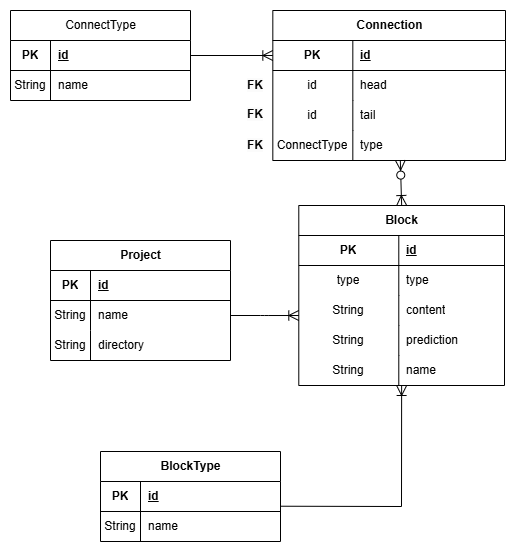
\includegraphics[width=0.8\textwidth]{images/DB block design.drawio.png}
	\caption{Block Relational Database Design}
	\label{fig:block-erd}
\end{figure}

\subsection{System Workflow}

\hspace{0.5cm}Test Genie's workflow implements a comprehensive process from source code intake to test generation, with specific mechanisms to address source code bias at each stage. The workflow proceeds through several distinct phases:

\subsubsection{Project Initialization}

\begin{enumerate}
    \item \textbf{Repository Acquisition}: The system clones the user-specified Git repository
    \item \textbf{Framework Detection}: Project structure is analyzed to identify the programming framework
    \item \textbf{Configuration Extraction}: Framework-specific configuration files are parsed to understand project organization
\end{enumerate}

\subsubsection{Source Code Analysis}

\begin{enumerate}
    \item \textbf{File Filtering}: Non-essential files (e.g., assets, configurations) are excluded from analysis
    \item \textbf{AST Generation}: Source files are parsed into abstract syntax trees
    \item \textbf{Block Identification}: The BLA algorithm identifies discrete functional blocks
    \item \textbf{Connection Mapping}: Relationships between blocks are discovered and cataloged
\end{enumerate}

\subsubsection{Business Logic Analysis}

\begin{enumerate}
    \item \textbf{Block-Level Analysis}: Each block is analyzed independently to focus on its specific purpose
    \item \textbf{Contextual Enrichment}: Block analysis is enhanced with limited information about connected blocks
    \item \textbf{Prediction Generation}: The system generates predictions about each block's business purpose
    \item \textbf{Prediction Storage}: Predictions are stored in the database for future reference and refinement
\end{enumerate}

\subsubsection{Human-in-the-Loop Refinement}

\begin{enumerate}
    \item \textbf{Visualization}: The block structure is visualized in the UI as a navigable graph
    \item \textbf{Prediction Review}: Users can inspect and refine the AI-generated predictions
    \item \textbf{Contextual Understanding}: The visualization helps users understand how blocks interact
    \item \textbf{Feedback Integration}: User corrections are stored and used in subsequent analysis
\end{enumerate}

\subsubsection{Test Generation}

\begin{enumerate}
    \item \textbf{Block Selection}: Users select specific blocks for test generation
    \item \textbf{Context Assembly}: The system gathers relevant information about the selected block and its connections
    \item \textbf{Test Strategy Determination}: Based on block type and prediction, appropriate testing strategies are selected
    \item \textbf{Test Case Generation}: The system generates test cases focused on validating the predicted business purpose
    \item \textbf{Test Validation}: Generated tests are checked for syntax correctness and executability
\end{enumerate}

\subsubsection{Test Refinement}

\begin{enumerate}
    \item \textbf{Test Preview}: Users can preview generated tests in the UI
    \item \textbf{Error Detection}: The system identifies and reports issues found during validation
    \item \textbf{Automated Correction}: When possible, the system automatically corrects identified issues
    \item \textbf{Test Finalization}: Users can download or copy the final test files for integration into their project
\end{enumerate}

\hspace{0.5cm}Throughout this workflow, the block-based approach systematically mitigates source code bias by:

\begin{itemize}
    \item Analyzing discrete functional units rather than entire codebases
    \item Focusing on predicted business purpose rather than implementation details
    \item Enabling human correction of predictions before test generation
    \item Generating tests that validate intended behavior rather than actual implementation
\end{itemize}

\hspace{0.5cm}This workflow represents a significant advancement over traditional approaches that either accept source code bias as inevitable or attempt to avoid it by limiting access to implementation details. By decomposing the codebase into manageable units and enabling human oversight of the analysis process, Test Genie achieves a more effective balance between automation and human expertise.

\subsection{Technical Implementation Details}

\subsubsection{Block Decomposition Strategy}

\hspace{0.5cm}Test Genie's approach to block decomposition balances granularity with semantic meaning. The system identifies blocks at several levels of abstraction:

\begin{itemize}
    \item \textbf{File-Level Blocks}: Represent entire source files, capturing overall purpose and structure
    \item \textbf{Class-Level Blocks}: Represent individual classes, encapsulating state and behavior
    \item \textbf{Method-Level Blocks}: Represent methods and functions, capturing specific behaviors
    \item \textbf{Nested Blocks}: Represent significant nested structures like inner classes or complex control flows
\end{itemize}

\hspace{0.5cm}This multi-level approach ensures that blocks maintain semantic coherence while remaining manageable for analysis. The system employs framework-specific heuristics to identify meaningful blocks. For Flutter, this includes recognition of widget classes, state classes, and business logic components.

\subsubsection{Prediction Generation Approach}

\hspace{0.5cm}The prediction generation process employs a two-phase approach:

\begin{enumerate}
    \item \textbf{Initial Analysis}: Each block is analyzed in isolation to generate a preliminary understanding of its purpose
    \item \textbf{Contextual Refinement}: Limited information about connected blocks is incorporated to refine the analysis
\end{enumerate}

\hspace{0.5cm}This approach balances the need for contextual understanding with the goal of avoiding source code bias. By limiting the contextual information to essential relationships rather than implementation details of connected blocks, the system maintains focus on business purpose over implementation mechanisms.

\hspace{0.5cm}The AI model used for prediction generation is enhanced with domain-specific knowledge through the vector stores, enabling more accurate interpretation of programming patterns and idioms. This enhancement is particularly important for framework-specific constructs, such as Flutter's widget hierarchy and state management patterns.

\subsubsection{Test Generation Strategy}

\hspace{0.5cm}Test Genie's test generation strategy focuses on validating the predicted business purpose of each block, implementing a three-phase approach:

\begin{enumerate}
    \item \textbf{Test Planning}: Based on the block's predicted purpose, the system identifies appropriate test scenarios
    \item \textbf{Test Structuring}: The system creates a framework-compliant test structure with appropriate setup and assertions
    \item \textbf{Test Validation}: Generated tests are validated for syntax correctness and executability
\end{enumerate}

\hspace{0.5cm}The test generation process deliberately avoids direct examination of the block's implementation details beyond what is necessary to establish method signatures and input/output types. This approach ensures that tests validate the expected behavior rather than merely confirming the current implementation.

\subsection{Addressing Source Code Bias Through System Design}

\hspace{0.5cm}Test Genie's architecture directly addresses the challenge of source code bias in AI-based test generation through several key mechanisms:

\begin{itemize}
    \item \textbf{Block-Based Decomposition}: By analyzing discrete functional units rather than entire codebases, the system reduces the complexity of each analysis task and focuses on specific business purposes rather than implementation interactions.
    
    \item \textbf{Separation of Prediction and Testing}: The system maintains a clear separation between the prediction of business purpose and the generation of tests, allowing each process to focus on its specific objective without contamination.
    
    \item \textbf{Human-in-the-Loop Refinement}: By enabling users to review and correct AI-generated predictions, the system leverages human expertise to identify cases where the AI has focused too heavily on implementation details rather than business intent.
    
    \item \textbf{Context-Limited Analysis}: The system deliberately limits the contextual information used in analysis to prevent over-reliance on implementation details of related components.
    
    \item \textbf{Validation-Focused Testing}: Tests are designed to validate the predicted business purpose rather than to verify the current implementation, ensuring that they provide meaningful quality assurance rather than tautological confirmation.
\end{itemize}

\hspace{0.5cm}These design choices represent a fundamental shift from traditional approaches to AI-based test generation. Rather than attempting to generate tests directly from implementation details or avoiding implementation details entirely, Test Genie embraces a middle path that leverages the strengths of both approaches while mitigating their weaknesses.

\hspace{0.5cm}By decomposing the codebase into manageable blocks, the system makes it feasible to analyze each component's intended purpose without being overwhelmed by implementation complexity. By enabling human oversight of the prediction process, the system leverages human expertise to correct cases where the AI has misinterpreted business intent. And by generating tests based on these refined predictions rather than implementation details, the system produces tests that provide genuine validation rather than merely confirming the current implementation.

\hspace{0.5cm}This approach offers several advantages over traditional methods:

\begin{enumerate}
    \item \textbf{Improved Test Quality}: Tests validate business requirements rather than implementation details, providing more meaningful quality assurance.
    
    \item \textbf{Enhanced Maintainability}: Tests remain valid even as implementations change, as long as the business purpose remains consistent.
    
    \item \textbf{Greater Transparency}: The separation of prediction and testing makes the system's reasoning process more interpretable and correctable.
    
    \item \textbf{More Efficient Human Oversight}: By decomposing the codebase into manageable blocks, the system makes it feasible for humans to review and correct AI-generated predictions.
\end{enumerate}

\hspace{0.5cm}Through these mechanisms, Test Genie's architecture effectively addresses the challenge of source code bias in AI-based test generation, offering a more effective and efficient approach to automated testing that balances AI capabilities with human expertise.

\subsection{Alignment with User Requirements}

\hspace{0.5cm}Test Genie's system design directly addresses the user requirements outlined in Table~\ref{tab:user-requirements}:

\begin{itemize}
    \item \textbf{Requirement 001 - Read project's source code}: The Project Manager module implements robust Git repository handling capabilities, supporting major hosting platforms.
    
    \item \textbf{Requirement 002 - Download/copy unit test/integration test}: The UI provides intuitive mechanisms for downloading or copying generated test files.
    
    \item \textbf{Requirement 003 - Interactive business logic analyzation}: The block visualization and prediction editing features enable effective human-in-the-loop participation.
    
    \item \textbf{Requirement 004 - Performance}: The block-based decomposition approach and efficient caching mechanisms ensure reasonable performance even for larger projects.
    
    \item \textbf{Requirement 005 - Test file correctly reflect business model}: The separation of prediction and testing ensures that tests validate business requirements rather than implementation details.
    
    \item \textbf{Requirement 006 - Validate generated test}: The embedded SDK integration ensures that generated tests are syntactically correct and executable.
\end{itemize}

\hspace{0.5cm}This comprehensive alignment demonstrates the effectiveness of the system design in addressing the identified user needs while simultaneously tackling the challenge of source code bias.

\subsection{Conclusion}

\hspace{0.5cm}Test Genie's system design represents a significant innovation in automated test generation, addressing the fundamental challenge of source code bias through a novel block-based decomposition approach. By analyzing discrete functional units, enabling human refinement of predictions, and generating tests based on business purpose rather than implementation details, the system produces more meaningful and effective tests than traditional approaches.

\hspace{0.5cm}The modular architecture, with its clear separation of concerns between UI, middleware, and backend services, provides a robust foundation for future enhancements and extensions. The current implementation, focused on the Flutter framework, demonstrates the viability of this approach while laying groundwork for expansion to additional programming environments.

\hspace{0.5cm}Through its innovative design and implementation, Test Genie advances the state of the art in automated testing, offering a more effective balance between AI capabilities and human expertise that addresses the limitations of previous approaches.